% ICD and AICD: Saliency-Guided Masking Augmentation for Visual Classifiers
% Mateusz Walo, Lublin University of Technology
%
% Compile with:
%   pdflatex main && bibtex main && pdflatex main && pdflatex main
%
% Style: NeurIPS 2024 (download neurips_2024.sty from https://neurips.cc)
% Fallback: comment \usepackage{neurips_2024} and use \documentclass{article}

\documentclass{article}

% ---- NeurIPS style (comment out if unavailable) ----
% \usepackage{neurips_2024}

% ---- Packages ----
\usepackage[utf8]{inputenc}
\usepackage[T1]{fontenc}
\usepackage{lmodern}
\usepackage{microtype}
\usepackage{hyperref}
\usepackage{url}
\usepackage{booktabs}
\usepackage{amsmath}
\usepackage{amssymb}
\usepackage{mathtools}
\usepackage{graphicx}
\usepackage{subcaption}
\usepackage{placeins}
\usepackage{xcolor}
\usepackage{natbib}
\usepackage{geometry}
\usepackage{verbatim}

\geometry{
  a4paper,
  left=2.5cm, right=2.5cm,
  top=2.5cm,  bottom=2.5cm,
}

% ---- Notation macros ----
\newcommand{\R}{\mathbb{R}}
\newcommand{\E}{\mathbb{E}}
\newcommand{\1}{\mathbf{1}}
\newcommand{\ie}{\textit{i.e.}}
\newcommand{\eg}{\textit{e.g.}}
\DeclareMathOperator*{\argmax}{arg\,max}
\DeclareMathOperator*{\argmin}{arg\,min}

% ---- Title ----
\title{Intelligent Coarse Dropout and Anti-ICD:\\Saliency-Guided Masking Augmentation for Visual Classifiers}

\author{%
  Mateusz Walo\\[4pt]
  \normalsize Department of Applied Mathematics,
  Faculty of Mathematics and Information Technology,\\
  \normalsize Lublin University of Technology,
  ul.~Nadbystrzycka~38, 20-618 Lublin, Poland\\
  \normalsize \texttt{mateusz.walo.datascience@gmail.com}
}

\date{}

\begin{document}

\maketitle

\begin{abstract}
Visual classifiers trained with standard augmentation pipelines tend to exploit
spurious correlations: background statistics, texture patterns, or scene-level
cues that happen to co-occur with class labels but do not reflect object
structure.  Conventional augmentation strategies, including random crops, colour
jitter, and policy-based methods such as RandAugment and AutoAugment, are
constructed without reference to what the model has actually learned, and so
offer no mechanism for targeting the specific shortcuts a given classifier has
acquired.

We present Intelligent Coarse Dropout (\textbf{ICD}) and its complement
Anti-ICD (\textbf{AICD}), two data augmentation methods that condition spatial
masking on the model's own class activation maps.  Standard coarse dropout
(cutout) hides rectangular regions chosen at random, erasing background as
readily as object.  ICD and AICD make this saliency-aware: they split the image
into a grid of tiles, score each tile by its mean saliency, and selectively
mask tiles by a percentile threshold.  ICD masks the highest-saliency
tiles, the regions the model already relies on, so that the classifier must
recruit additional cues.  AICD masks the lowest-saliency tiles, perturbing the
background while leaving the discriminative region intact.  Masked tiles are
not filled with a hard black box but with one of several soft strategies
(blurred original, local mean, noise, or a constant), which preserve different
aspects of local context.

We describe the formal construction of both masks, the family of fill
strategies, the role of the tile size and threshold hyperparameters, and a
reference implementation in the open-source BNNR library.  This paper
introduces the methods; a quantitative evaluation against standard augmentation
baselines is left to a companion study.

\end{abstract}

\section{Introduction}
\label{sec:intro}

Convolutional neural networks trained on natural image datasets develop
systematic biases toward low-level texture features over global
shape~\citep{geirhos2019texture}.  On fine-grained datasets the effect is
pronounced: classifiers readily latch onto contextual cues such as the grass
behind a terrier, the greenhouse behind a flower, or the sky behind an
aircraft.  These correlations hold in the training distribution and can yield
high validation accuracy, yet they transfer poorly to images where the shortcut
is absent and leave the model brittle under distribution shift.

Data augmentation is the standard remedy.  The prevailing approach applies a
fixed family of photometric and geometric transformations uniformly throughout
training.  AutoAugment~\citep{cubuk2019autoaugment} and its descendants,
RandAugment~\citep{cubuk2020randaugment} and
TrivialAugment~\citep{muller2021trivialaugment}, search over large
transformation spaces but treat the network as a black box: the policy is fixed
before training and never consults the model's internal state.  Spatial-masking
regularisers such as Cutout~\citep{devries2017cutout} and Random
Erasing~\citep{zhong2020randomerasing} remove rectangular regions to discourage
reliance on any single patch, but the location of the mask is chosen uniformly
at random.  A random mask is blind to content; it deletes empty background as
often as it deletes the object.

This raises a natural question.  If a saliency method can tell us which regions
the model currently treats as discriminative, can we place the mask there
deliberately?  KeepAugment~\citep{gong2021keepaugment} explores one side of
this idea by \emph{protecting} high-saliency regions from augmentation, on the
premise that preserving informative content helps accuracy.  We examine the
complementary operations.  What happens when the high-saliency regions are
\emph{removed}, forcing the classifier to find evidence elsewhere?  And what
happens when only the low-saliency regions, the background and irrelevant
texture, are removed, concentrating the perturbation away from the object?

We formalise both operations as augmentation methods.  \textbf{Intelligent
Coarse Dropout (ICD)} masks the highest-saliency tiles of each input;
\textbf{Anti-ICD (AICD)} masks the lowest-saliency tiles.  Both derive their
masks from a GradCAM~\citep{selvaraju2017gradcam} saliency map evaluated at the
model's current parameters, so the augmentation tracks what the model has
learned at each stage of training.  Crucially, the masking decision is made at
the level of coarse tiles rather than individual pixels: the image is divided
into an $8\times 8$-pixel grid (by default), each tile is scored by its mean
saliency, and tiles are masked by a percentile threshold.  Coarse tiling makes
the mask robust to the high-frequency noise that pixel-level saliency maps
often exhibit, while keeping the masked region spatially coherent.  Rather than
a hard black rectangle, masked tiles are filled with a soft strategy: a blurred
copy of the original, a local or global mean colour, matched noise, or a
constant.  The surrounding context then degrades gracefully.

The contributions of this paper are as follows.
\begin{enumerate}
  \item We introduce ICD and AICD, two saliency-conditioned coarse-dropout
    augmentations, and give the formal tile-based mask construction together
    with the percentile-threshold rule that distinguishes them.
  \item We describe five fill strategies for masked tiles and characterise how
    each alters the information that remains available to the model.
  \item We discuss the methods' expected behaviour in terms of curriculum
    learning and spurious-correlation removal, and situate them with respect to
    random masking and saliency-protecting augmentation.
  \item We document a reference implementation in the open-source BNNR
    library~\citep{walo2026bnnr}, including the use of a precomputed saliency
    cache that makes online application practical.
\end{enumerate}

This paper is concerned with the methods themselves.  A controlled empirical
comparison of ICD and AICD against RandAugment, TrivialAugment, and AutoAugment,
together with the accompanying benchmark protocol, is the subject of a separate
study.

\section{Related Work}
\label{sec:related}

\paragraph{Masking augmentations.}
Cutout~\citep{devries2017cutout} removes a fixed-size square at a random
location and was among the first to show that occluding contiguous regions acts
as an effective regulariser.  Random Erasing~\citep{zhong2020randomerasing}
generalises this to rectangles of random aspect ratio and area, optionally
filled with noise or the dataset mean.  Both choose the masked region without
regard to image content.  ICD can be viewed as a content-aware Cutout: the
shape of the occlusion follows the model's saliency rather than a random box,
and the special case of solid zero-fill on the high-saliency tiles recovers a
saliency-targeted form of classical Cutout.  CutMix~\citep{yun2019cutmix}
replaces a region with a patch from a second image and mixes the labels
accordingly; unlike CutMix, ICD and AICD are single-image operations and leave
the label unchanged.

\paragraph{Saliency-aware augmentation.}
The closest line of work conditions augmentation on a saliency or attention
signal.  KeepAugment~\citep{gong2021keepaugment} computes a saliency map and
\emph{preserves} the most important region, restricting augmentation to the
remainder, with the goal of not destroying discriminative information.  ICD
adopts the opposite stance: it deliberately occludes the high-saliency region
to discourage over-reliance on it, while AICD occupies the same regime as
KeepAugment by perturbing only the low-saliency background.  The two methods
thus bracket the design space that KeepAugment occupies on one side.  Other
saliency-driven approaches operate through mixing rather than dropout:
SaliencyMix~\citep{uddin2021saliencymix} uses a saliency map to choose the
source patch in a CutMix-style operation, and SnapMix~\citep{huang2021snapmix}
uses class activation maps to assign mixed-label proportions in fine-grained
recognition.  These methods require a second image and modify the target;
ICD and AICD do neither.

\paragraph{Class activation maps.}
ICD and AICD rely on a saliency map to score image regions.  We use
GradCAM~\citep{selvaraju2017gradcam}, which weights the activations of a target
convolutional layer by the gradient of the predicted class score and produces a
coarse localisation map.  Numerous refinements exist, including
GradCAM\texttt{++}~\citep{chattopadhay2018gradcampp} for improved localisation
of multiple instances and gradient-free variants such as
EigenCAM~\citep{muhammad2020eigencam}, and any of these may in principle drive
the masking.  Our reference implementation builds on the
\texttt{pytorch-grad-cam} library~\citep{gildenblat2021gradcam}, which unifies
these methods behind a common interface.

\paragraph{Automated augmentation policies.}
A parallel body of work searches for augmentation policies rather than
conditioning on the model state.  AutoAugment~\citep{cubuk2019autoaugment}
learns a policy by reinforcement learning;
RandAugment~\citep{cubuk2020randaugment} reduces the search to two scalar
hyperparameters; and TrivialAugment~\citep{muller2021trivialaugment} dispenses
with search entirely, sampling a single transformation per image uniformly.
These methods are complementary to ICD and AICD: they define \emph{which}
photometric or geometric transformation to apply, whereas ICD and AICD define
\emph{where} to apply a content-aware occlusion.  The two can be composed.

\section{Method}
\label{sec:method}

ICD and AICD share a common construction.  Given a training image and the
classifier in its current state, we compute a saliency map, reduce it to a grid
of tile scores, threshold those scores to obtain a binary mask, and replace the
masked tiles with a fill.  The two methods differ only in the direction of the
threshold.  We describe each step in turn.

\subsection{Saliency Map}
\label{sec:method:saliency}

Let $f_\theta : \mathcal{X} \to \R^{C}$ be a classifier with parameters
$\theta$ over $C$ classes, and let $l$ index a chosen convolutional layer with
feature maps $A^{k,l} \in \R^{h_l \times w_l}$, $k = 1,\dots,K_l$.  Each image
carries a target class $y$ at which the saliency is computed; by default $y$ is
the ground-truth label of the training image, though the model's prediction
$\argmax_c f_\theta(x)_c$ may be substituted.  For an input
$x \in \R^{H \times W \times 3}$ the GradCAM~\citep{selvaraju2017gradcam}
saliency map is
\begin{equation}
  S_\theta(x,y)
  \;=\;
  \mathrm{ReLU}\!\left( \sum_{k=1}^{K_l} \alpha_k^{y}\, A^{k,l} \right),
  \qquad
  \alpha_k^{y}
  \;=\;
  \frac{1}{h_l w_l} \sum_{i=1}^{h_l} \sum_{j=1}^{w_l}
  \frac{\partial\, f_\theta(x)_{y}}{\partial\, A^{k,l}_{ij}} .
  \label{eq:gradcam}
\end{equation}
The rectifier discards activations that argue against class $y$.  The resulting
map is upsampled bilinearly to the input resolution $(H,W)$ and rescaled to
$[0,1]$; we write $S_\theta(x,y) \in [0,1]^{H \times W}$ for this normalised
map.  The reference implementation (Section~\ref{sec:implementation}) applies
the eigen-smoothing variant of this map by default, taking the saliency as the
first principal component of the gradient-weighted activations rather than their
plain sum, which suppresses high-frequency artefacts.  Either form may be used
to drive the masking that follows.

\subsection{Tile Scoring}
\label{sec:method:tiles}

Pixel-level saliency maps are noisy, and masking individual pixels would
produce a fragmented, high-frequency occlusion.  We instead aggregate the map
over a regular grid.  Fix a tile size $t \in \mathbb{Z}_{>0}$ and form
$n_r = \lfloor H/t \rfloor$ rows and $n_c = \lfloor W/t \rfloor$ columns of
non-overlapping $t \times t$ tiles, discarding any boundary strip that does not
divide evenly.  The score of tile $(a,b)$ is the mean saliency over its pixels,
\begin{equation}
  T_{ab}
  \;=\;
  \frac{1}{t^2}
  \sum_{p=at}^{(a+1)t - 1} \;\sum_{q=bt}^{(b+1)t - 1}
  \big[ S_\theta(x,y) \big]_{pq},
  \qquad
  a \in \{0,\dots,n_r{-}1\},\;\,
  b \in \{0,\dots,n_c{-}1\},
  \label{eq:tilescore}
\end{equation}
yielding a score matrix $T \in \R^{n_r \times n_c}$.

\subsection{Thresholding: ICD and AICD}
\label{sec:method:threshold}

Let $\rho \in (0,1)$ be a percentile parameter and let $Q_\rho(T)$ denote the
$\rho$-quantile of the flattened tile scores $\{T_{ab}\}$.  The two methods
threshold $T$ in opposite directions.

\paragraph{ICD (Intelligent Coarse Dropout)} masks the tiles whose saliency
exceeds the $\rho$-quantile, that is, the most salient tiles:
\begin{equation}
  M^{\mathrm{ICD}}_{ab}
  \;=\;
  \1\!\left[\, T_{ab} > Q_\rho(T) \,\right].
  \label{eq:icdmask}
\end{equation}

\paragraph{AICD (Anti-ICD)} masks the tiles whose saliency falls below the
$(1{-}\rho)$-quantile, that is, the least salient tiles:
\begin{equation}
  M^{\mathrm{AICD}}_{ab}
  \;=\;
  \1\!\left[\, T_{ab} < Q_{1-\rho}(T) \,\right].
  \label{eq:aicdmask}
\end{equation}

Both masks select, in expectation, the same fraction $1-\rho$ of all tiles:
ICD takes the top $1-\rho$, AICD the bottom $1-\rho$.  With the default
$\rho = 0.70$ each method masks roughly $30\%$ of the tiles.  This symmetry is
deliberate, since it lets the two methods be compared at matched occlusion area.
The masks are exact complements only in the limiting case $\rho = 0.5$; for
$\rho > 0.5$ a neutral band of mid-saliency tiles is left untouched by both.

The binary tile mask is expanded to pixel resolution by repeating each tile
decision across its $t \times t$ block,
\begin{equation}
  \widehat{M}_{pq} \;=\; M_{\lfloor p/t \rfloor,\, \lfloor q/t \rfloor},
  \label{eq:upsample}
\end{equation}
with any discarded boundary strip left unmasked, giving
$\widehat{M} \in \{0,1\}^{H \times W}$.

\subsection{Fill}
\label{sec:method:fill}

A masked tile must be replaced by something.  Rather than the hard black box of
classical Cutout, we substitute a fill $\phi(x) \in \R^{H \times W \times 3}$,
applied only inside the mask:
\begin{equation}
  \tilde{x}
  \;=\;
  \big(1 - \widehat{M}\big) \odot x
  \;+\;
  \widehat{M} \odot \phi(x),
  \label{eq:fill}
\end{equation}
where $\odot$ is element-wise multiplication broadcast over channels.  We
provide five choices of $\phi$, summarised in Table~\ref{tab:fills}.  The
default, \texttt{gaussian\_blur}, replaces masked pixels with a strongly blurred
copy of the image (kernel size set to the nearest odd integer to $0.15 \cdot
\max(H,W)$); this removes local detail while retaining coarse colour and
luminance, so the occlusion is visible to the network without introducing a
sharp artificial edge.  The \texttt{solid} strategy with a zero value recovers
classical Cutout~\citep{devries2017cutout}, here restricted to the
saliency-selected tiles.

\begin{table}[t]
\centering
\caption{Fill strategies for masked tiles.  Each defines the function
$\phi(\cdot)$ in Eq.~\eqref{eq:fill}.}
\label{tab:fills}
\small
\begin{tabular}{@{}lll@{}}
\toprule
Strategy & $\phi(x)$ on masked pixels & Effect \\
\midrule
\texttt{gaussian\_blur} & blurred copy of $x$, $\sigma \propto \max(H,W)$ & removes detail, keeps coarse colour (default) \\
\texttt{local\_mean}    & mean colour of neighbouring unmasked tiles      & smooth, locally consistent fill \\
\texttt{global\_mean}   & per-channel global mean of $x$                  & flat region, no local cue \\
\texttt{noise}          & Gaussian noise matched to per-channel stats     & high-frequency perturbation \\
\texttt{solid}          & constant value (default $0$)                    & hard masking; recovers Cutout for $M^{\mathrm{ICD}}$ \\
\bottomrule
\end{tabular}
\end{table}

\subsection{Illustration}
\label{sec:method:illustration}

Figure~\ref{fig:comparison} shows the full construction on four images.  The
second column is the GradCAM map of Eq.~\eqref{eq:gradcam}; the third applies
ICD, blurring the region the model attends to; the fourth applies AICD, blurring
everything else.  The same saliency map drives both augmentations.  In the
Labrador and cat rows the network localises the face, so ICD blurs the face and
AICD blurs the surrounding fur and background; in the espresso row the saliency
concentrates on the cup rim, and in the sports-car row on the lower body of the
car, with the two augmentations partitioning the image accordingly.

\begin{figure}[ht]
\centering
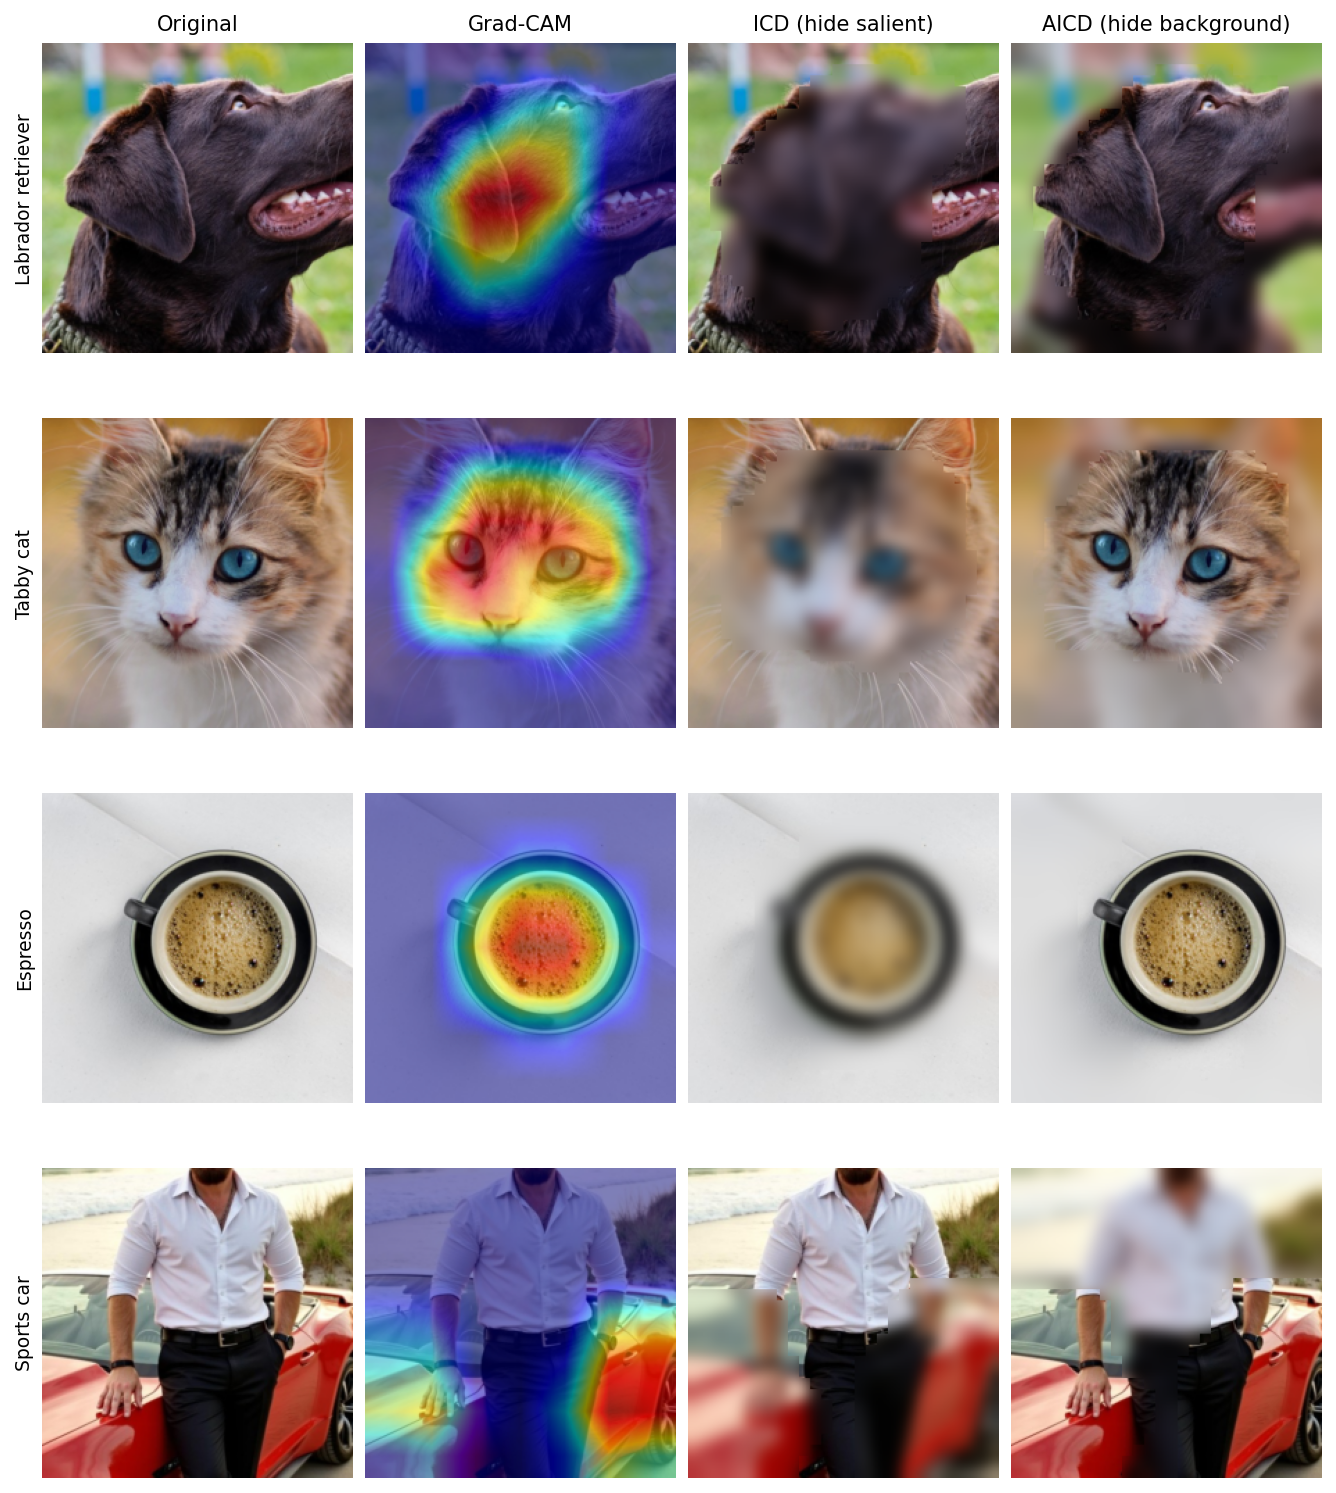
\includegraphics[width=0.72\linewidth]{figures/icd_aicd_comparison.png}
\caption{The ICD/AICD construction on four ImageNet classes.  From left to
right: the original image; the GradCAM saliency map at the final convolutional
layer of a ResNet-18; ICD, which masks the highest-saliency tiles
(Eq.~\ref{eq:icdmask}); and AICD, which masks the lowest-saliency tiles
(Eq.~\ref{eq:aicdmask}).  Both use $\rho = 0.5$ for clear visualisation and a
Gaussian-blur fill.  The same saliency map produces both masks.}
\label{fig:comparison}
\end{figure}

Figure~\ref{fig:fills} fixes the mask and varies the fill, illustrating the
qualitative difference between the strategies of Table~\ref{tab:fills} for both
ICD (top) and AICD (bottom).  Figure~\ref{fig:tiles} varies the tile size $t$:
small tiles trace the saliency contour closely but fragment the occlusion,
whereas large tiles produce a coarse, block-structured mask that is less
sensitive to saliency noise.

\begin{figure}[ht]
\centering
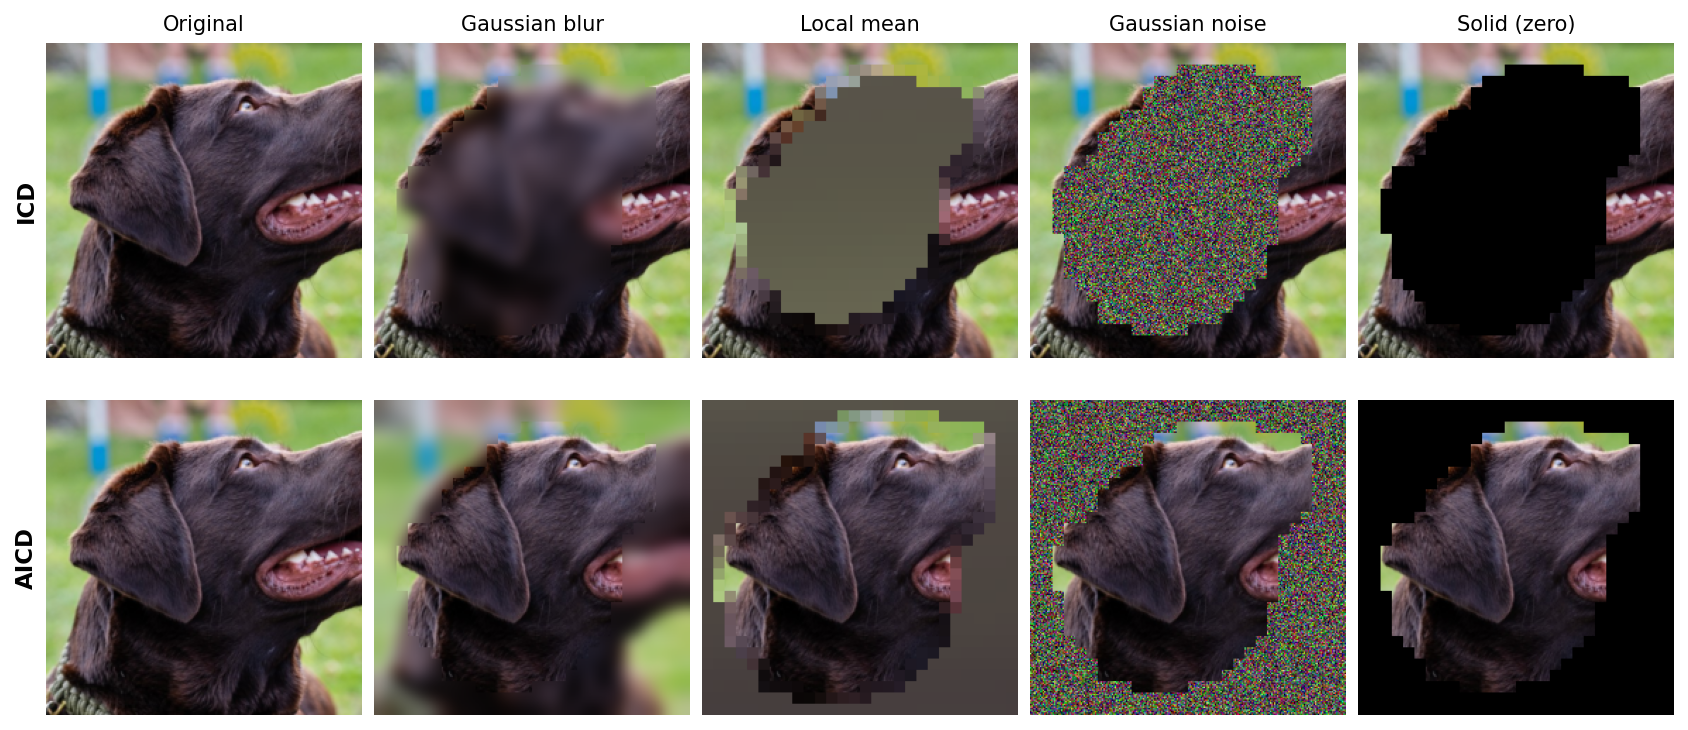
\includegraphics[width=0.92\linewidth]{figures/fill_strategies.png}
\caption{Four of the five fill strategies of Table~\ref{tab:fills} (the
\texttt{global\_mean} strategy is omitted for space) applied under a fixed mask,
for ICD (top row) and AICD (bottom row) on the same image.  Gaussian blur is the
default soft fill; local mean and noise preserve different aspects of the
original content; solid zero-fill is the hard limit and reduces to classical
Cutout.}
\label{fig:fills}
\end{figure}

\begin{figure}[ht]
\centering
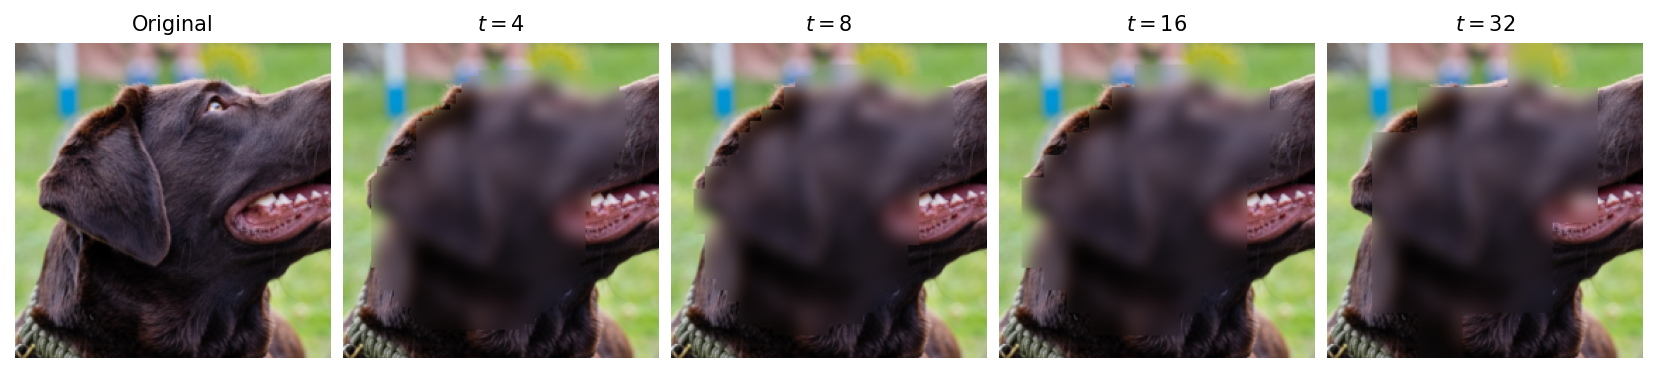
\includegraphics[width=0.92\linewidth]{figures/tile_sizes.png}
\caption{Effect of the tile size $t$ on the ICD mask (Gaussian-blur fill,
$\rho = 0.5$).  Smaller tiles follow the saliency map more closely at the cost
of a fragmented occlusion; larger tiles yield a coarser, more contiguous mask.}
\label{fig:tiles}
\end{figure}

\subsection{Hyperparameters}
\label{sec:method:hparams}

The construction has three principal hyperparameters.  The percentile $\rho$
sets the masked fraction $1-\rho$: larger $\rho$ masks fewer, more selective
tiles.  The tile size $t$ trades spatial fidelity for robustness, as in
Figure~\ref{fig:tiles}.  The fill $\phi$ determines what the network sees in
place of the occluded content.  In addition, each augmentation is applied
stochastically with probability $p$ per image, returning the image unchanged
with probability $1-p$; this keeps a fraction of clean images in every batch.
The library defaults are $t = 8$, Gaussian-blur fill, and a percentile of
$\rho = 0.70$; we set $p = 0.5$ for training so that half of each batch is
clean.  A lower $\rho$ is used only for the visualisations in this paper, where
a larger masked area is easier to read.

\FloatBarrier

\section{Discussion}
\label{sec:discussion}

We motivate ICD and AICD through two distinct mechanisms, and then note the
assumptions and costs that the construction carries.

\subsection{ICD as model-adaptive difficulty}
\label{sec:discussion:icd}

ICD removes exactly the evidence the model currently finds most convincing.
Consider a classifier that has settled on a single dominant cue, such as a dog's
face or a flower's centre.  Under ICD it repeatedly encounters that cue occluded
and must predict from what remains.  This is a form of difficulty that adapts to the
model rather than to the data: the same image presents a harder problem to a
network that relies narrowly on one region than to one that already integrates
several.  The mechanism is related to the motivation of
curriculum learning~\citep{bengio2009curriculum}, with the ordering inverted.
Where a curriculum presents easy examples first and hard examples later, ICD
holds the data fixed and instead removes, at each step, whatever the model has
found easy.  The target it removes therefore moves, defined by the model's own
saliency.  Because the
saliency in Eq.~\eqref{eq:gradcam} is recomputed from the current parameters,
the occlusion follows the representation as it develops rather than being fixed
in advance.

\subsection{AICD as background suppression}
\label{sec:discussion:aicd}

AICD addresses the complementary failure mode.  In many natural datasets the
background is statistically informative: water co-occurs with certain animals,
indoor scenes with certain objects~\citep{beery2018recognition}.  A model can
exploit this without ever attending to the object, and such reliance is
invisible to validation accuracy when the validation set shares the same
background statistics.  AICD masks precisely the low-saliency region, which is
the background once the model has localised the object, and perturbs it
with a fill.  Repeatedly altering the background while preserving the object
discourages the classifier from treating background as evidence, in the spirit
of work that removes or randomises background to test and improve object-level
reliance~\citep{xiao2021noise}.

\subsection{Expected effect on saliency}
\label{sec:discussion:saliency}

Both methods act on the saliency map and may, in turn, reshape it.  Suppressing
the high-saliency region (ICD) should discourage the concentration of saliency
on any single area, so we would expect a model trained with ICD to develop a
more distributed saliency map; suppressing the background (AICD) should, if it
succeeds, sharpen saliency onto the object.  These expectations are stated here
as hypotheses.  Quantitative measures such as the fraction of saliency mass on
the image border, the coverage above a threshold, and the Gini concentration of
the map can make them testable, and we take up that measurement in the companion
study rather than claiming any outcome here.

\subsection{Assumptions and limitations}
\label{sec:discussion:limits}

The construction rests on several assumptions that bound its applicability.

\paragraph{Saliency must be meaningful.}
ICD and AICD are only as good as the saliency map that drives them.  At
initialisation, before the network has learned useful features, the GradCAM map
is close to uninformative, and masking by it approaches random masking.  The
methods are therefore best applied once the model has partially trained, or with
saliency computed from a warmed-up checkpoint; applying them from the first step
is unlikely to differ from Cutout.

\paragraph{Online cost.}
Unlike dataset-level augmentations that can be precomputed, the saliency in
Eq.~\eqref{eq:gradcam} depends on the current parameters and in principle must
be recomputed as training proceeds.  A gradient evaluation per image per update
is expensive.  Section~\ref{sec:implementation} describes the caching strategy
we use to amortise this, but the cache trades freshness for speed: a cached map
reflects the model at the time of caching, not the current step.

\paragraph{Tile granularity.}
The tile size $t$ is a fixed grid imposed on a continuous saliency map.  A small
$t$ can mask fine object parts that happen to be salient; a large $t$ can mask
substantial background along with the object.  The appropriate $t$ depends on
the object scale relative to the image, which the method does not adapt
automatically.

\paragraph{Single-image, single-label scope.}
ICD and AICD operate on one image and leave the label unchanged, which keeps
them simple and composable but also means they do not exploit the label-mixing
that benefits methods such as CutMix~\citep{yun2019cutmix} and
SnapMix~\citep{huang2021snapmix}.  The construction as presented is specific to
classification; extending the tile-scoring step to detection or segmentation,
where saliency is defined per region or per pixel, is left to future work.

\section{Implementation}
\label{sec:implementation}

ICD and AICD are implemented in the open-source BNNR
library~\citep{walo2026bnnr} (MIT licensed, available on PyPI as
\texttt{bnnr}).  The saliency back end is the
\texttt{pytorch-grad-cam} package~\citep{gildenblat2021gradcam}, so the maps of
Eq.~\eqref{eq:gradcam} come from a standard, widely used GradCAM implementation
rather than a bespoke one; by default the library enables that package's
eigen-smoothing option, as noted in Section~\ref{sec:method:saliency}.  This
section describes how the methods are applied during training.

\subsection{Online application and the saliency cache}
\label{sec:implementation:cache}

Because the saliency map depends on the current parameters, a naive
implementation would run a GradCAM pass for every image at every step, roughly
doubling the cost of training.  BNNR amortises this with a disk-backed cache.
Before a training run (or after a warm-up phase, as discussed in
Section~\ref{sec:discussion:limits}), the saliency map for each training image
is computed once and stored, keyed by a hash of the image content:
\begin{verbatim}
    from bnnr.xai_cache import XAICache
    cache = XAICache("./xai_cache")
    cache.precompute_cache(
        model=model,
        train_loader=train_loader,   # yields (image, label, index)
        target_layers=target_layers, # e.g. [model.layer4[-1]]
        n_samples=len(train_dataset),
        method="gradcam",
    )
\end{verbatim}
During training the augmentations read tile masks from the cache instead of
recomputing GradCAM, reducing the per-step overhead to a cache lookup and the
masking arithmetic of Eqs.~\eqref{eq:tilescore}--\eqref{eq:fill}.  The cache
reflects the model at the time of precomputation; refreshing it periodically
trades additional compute for saliency that tracks the evolving model more
closely.

\subsection{Use in a training loop}
\label{sec:implementation:loop}

The augmentations are plain callables that take a batch and its labels.  A
classification step looks as follows:
\begin{verbatim}
    from bnnr.icd import ICD, AICD
    icd  = ICD(model=model,  target_layers=target_layers,
               cache=cache,  threshold_percentile=70.0,
               tile_size=8,  fill_strategy="gaussian_blur",
               probability=0.5)
    aicd = AICD(model=model, target_layers=target_layers,
                cache=cache, threshold_percentile=70.0)

    for images, labels, index in train_loader:   # images uint8 NHWC
        images = icd.apply_batch_with_labels(
            images, labels, sample_indices=index)
        # ... convert to [0,1] BCHW, forward, backward, step ...
\end{verbatim}
The label passed to the augmentation is the class whose saliency defines the
mask; by default this is the ground-truth label, though the model's prediction
may be used instead.  The \texttt{DataLoader} yields a sample index as a third
element so the cache can retrieve the correct precomputed map.  Images are
expected in $[0,1]$ (or uint8, converted internally); ImageNet normalisation, if
used, is applied after the augmentation so that the saliency back end and the
fill operate on unnormalised pixels.

ICD and AICD are independent augmentations and need not be used together.  Each
can be inserted into any existing PyTorch loop, including framework wrappers such
as Lightning, without further dependencies, and either can be composed
with conventional augmentations (random crop, flip, colour jitter) applied
before or after the masking step.

\section{Conclusion}
\label{sec:conclusion}

We have presented Intelligent Coarse Dropout (ICD) and Anti-ICD (AICD), two
augmentation methods that turn a GradCAM saliency map into a tile-based
occlusion mask.  ICD masks the tiles the model finds most salient, removing the
evidence it currently relies on; AICD masks the least salient tiles, perturbing
the background while leaving the discriminative region intact.  The two are
governed by a single percentile threshold that selects them as opposite
directions of the same construction and fixes their occlusion area to a common
fraction.  Masked tiles are replaced by one of several soft fills rather than a
hard box, and the masking operates at a coarse tile granularity that tempers the
noise of pixel-level saliency.  The methods are implemented in the open-source
BNNR library on top of \texttt{pytorch-grad-cam}, with a saliency cache that
makes their online use practical.

The present paper introduces the methods and their rationale; it makes no
empirical claim about their effect on accuracy.  The natural next step is a
controlled comparison of ICD and AICD against RandAugment, TrivialAugment,
AutoAugment, and random masking, under matched compute and a held-out test
split.  That comparison, together with the saliency measurements proposed in
Section~\ref{sec:discussion:saliency}, would test whether the methods reshape the
model's attention as their design intends.  We report that study separately.
Further directions include adapting the tile size to object scale, refreshing
the saliency cache on a schedule, substituting alternative class activation
methods for GradCAM, and extending the tile-scoring construction beyond
classification to detection and segmentation.


\bibliographystyle{abbrvnat}
\bibliography{refs}

\end{document}
